\section{\textsc{Gewienertes Omlett}}

\subsection*{Zutaten für 1 Omlett:}

\begin{tabular}{p{7.5cm} p{7.5cm}}
	& \\
	4 Eier & 2 Wiener Würstchen \\
	\sfrac{1}{2} Zwiebel & 200g Mozzarella \\
	Salz und Pfeffer &
\end{tabular}

\subsection*{Serviervorschlag:}

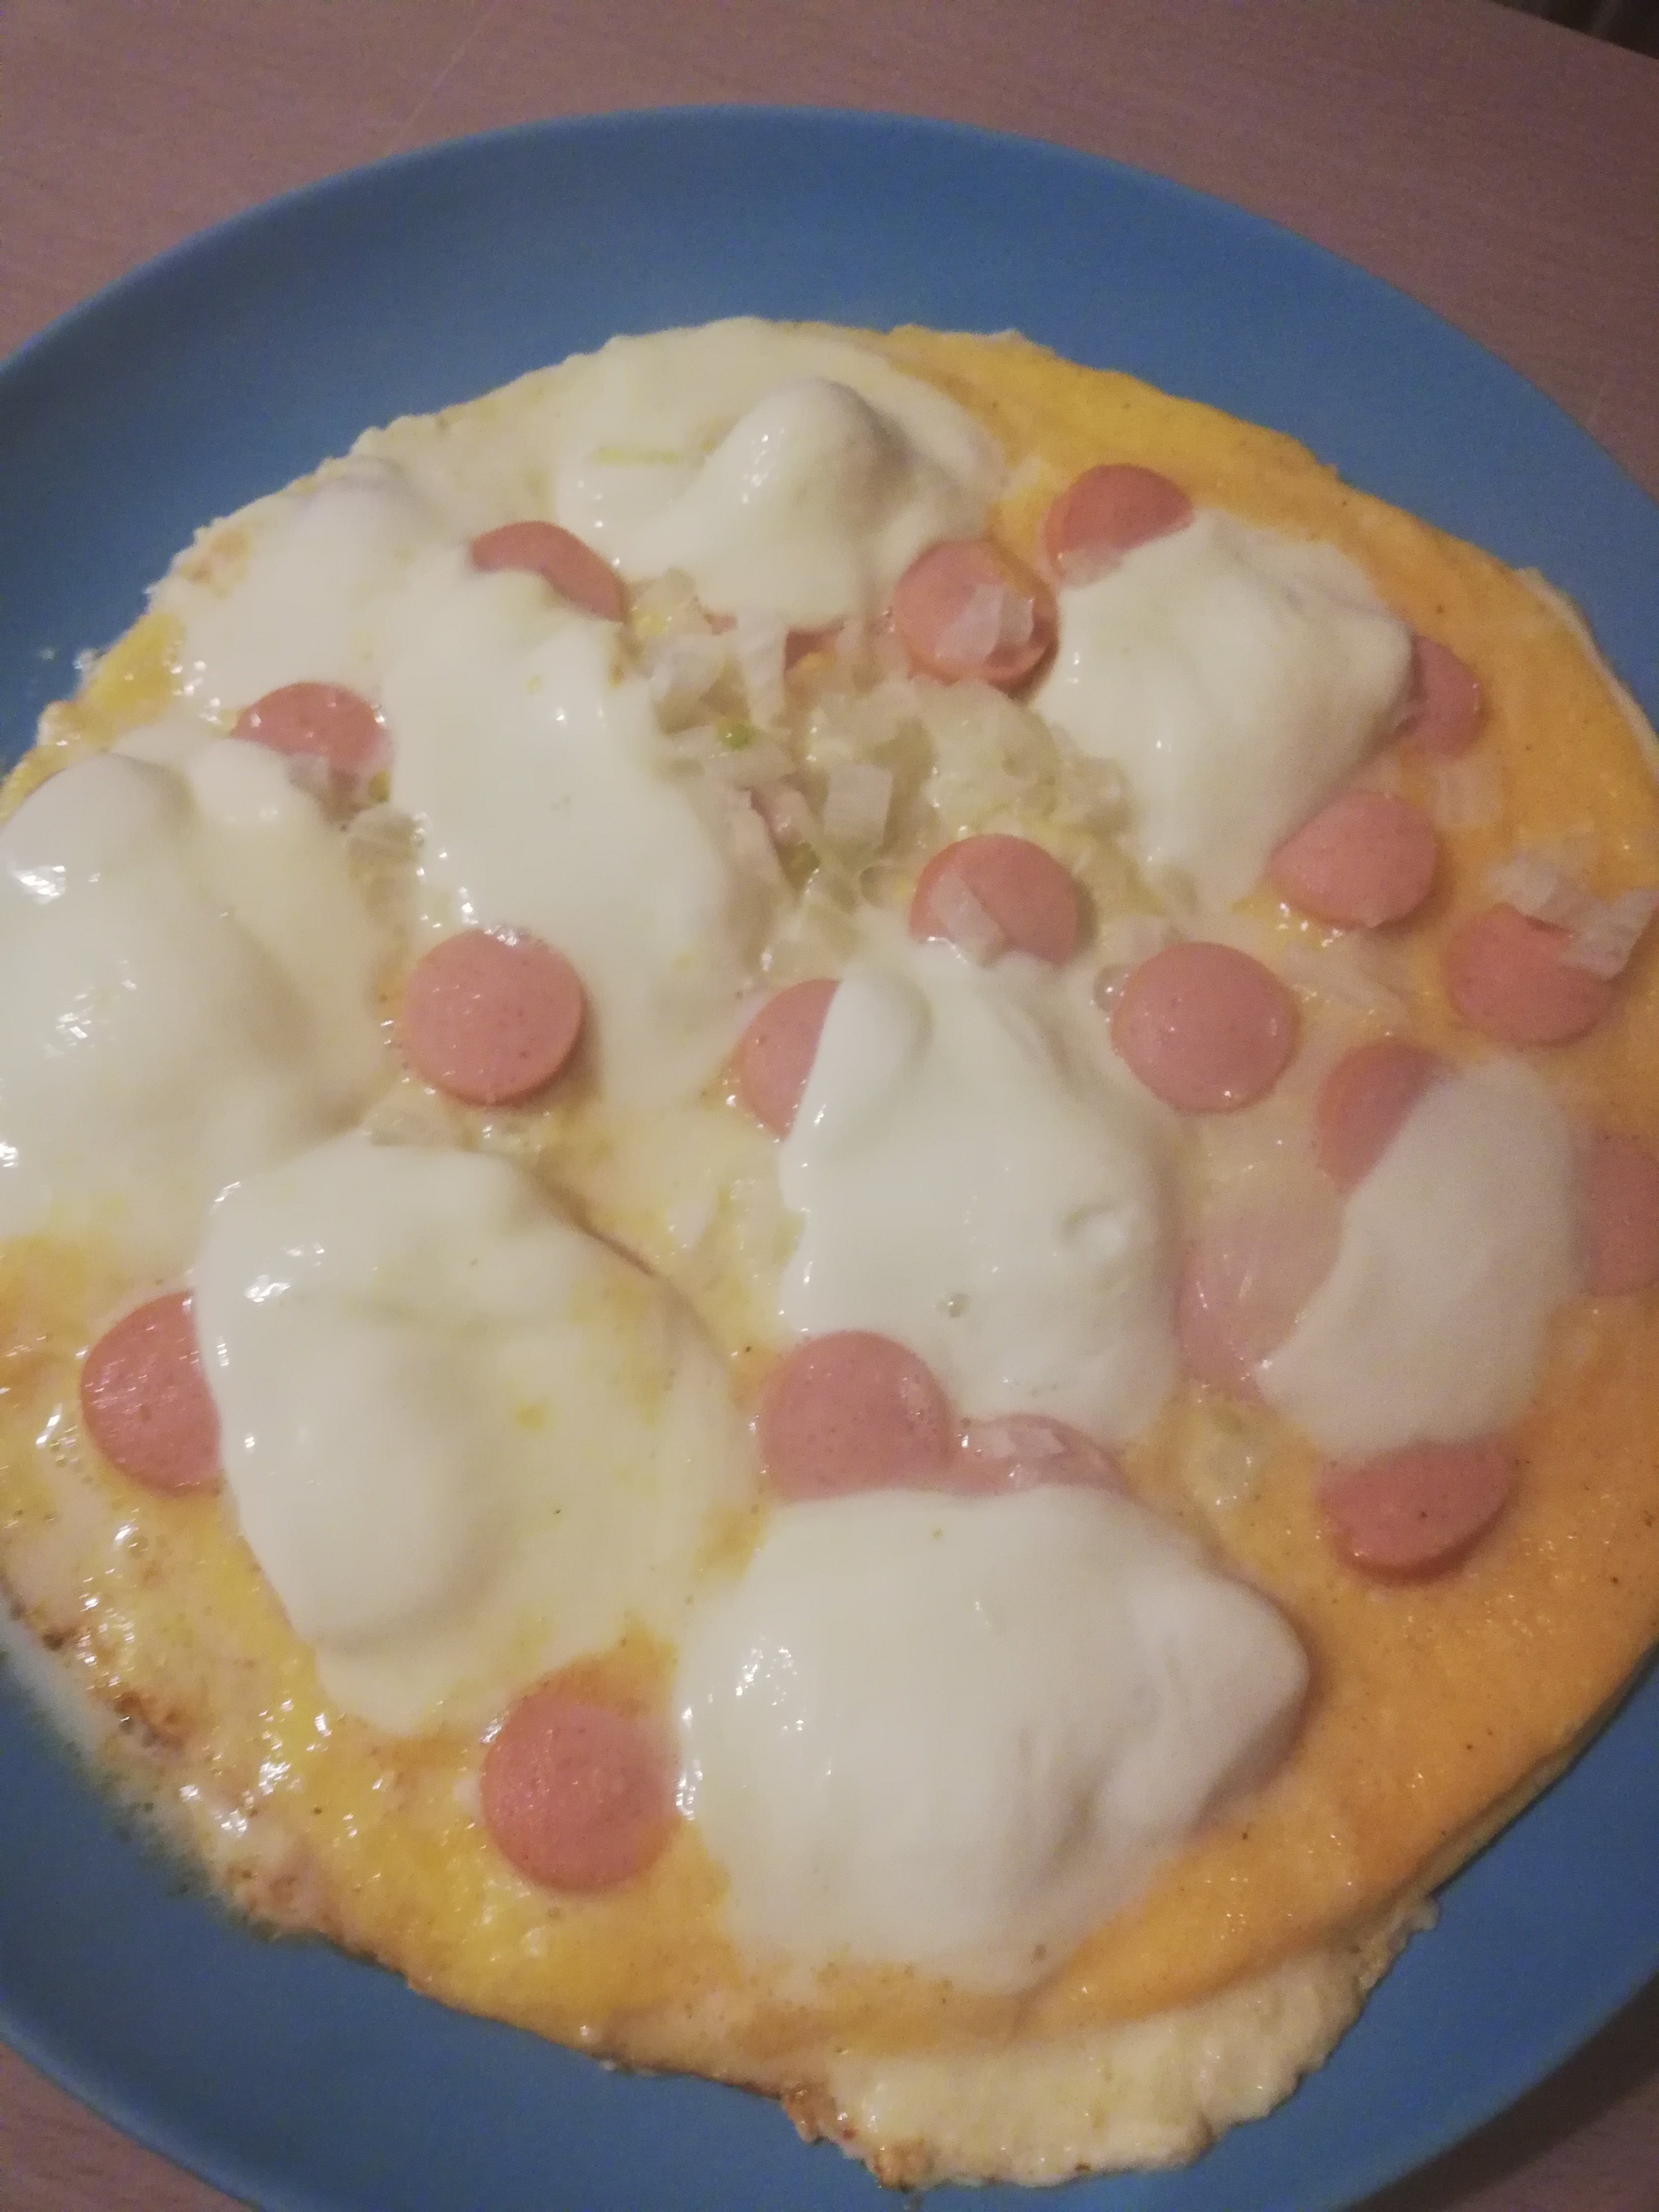
\includegraphics[width=\textwidth]{img/omlett/omlett_wiener_fertig.jpg} \cite{omlettwiener}

\subsection*{So geht's}

\begin{tabular}{p{15cm}}
	Die Eier in eine Schüssel aufschlagen und schaumig schlagen.\\
	In einer großen Pfanne die Butter schmelzen.\\
	In der Zwischenzeit die Wiener in dünne Scheiben schneiden.\\
	Die Zwiebeln fein würfeln.\\
	Die Eimasse in die Pfanne geben und auf großer Hitze stocken lassen.\\
	Die Wiener und die Zwiebeln auf dem Omlett verteilen.\\
	Mit einem Deckel auf der Pfanne 5min braten.\\
	Auf einem großen Teller servieren.
\end{tabular}
